\documentclass[a4paper]{article}

\usepackage{array}
\usepackage{placeins}

\usepackage{hopsantut}

\begin{document}
\maketitle{Exporting Models to Simulink}

\section*{Introduction}
Bla bla introduktion

\section*{Requirements}
%Matlab/Simulink
%VC++ (rätt version, eroende på version av Matlab)

\begin{enumerate}
\tutitem{Do the first thing}
Explain how to do the first thing

%Öppna position servo (bild)
 
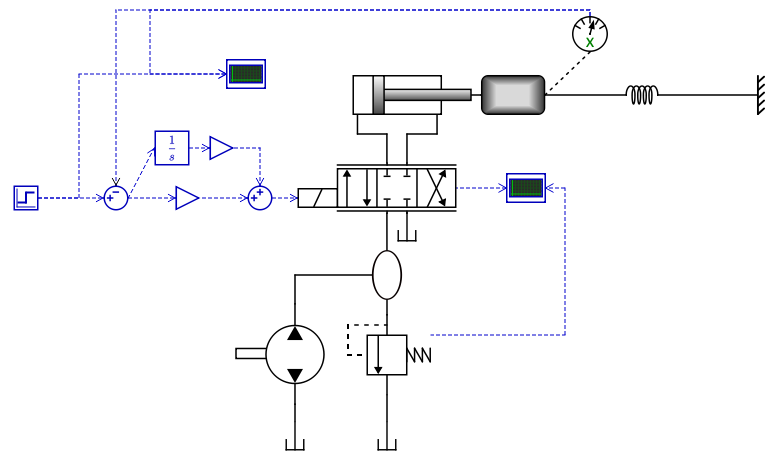
\includegraphics[height=7cm]{gfx/simulink/model1.png}
 
%Ta bort regulatorn (bild)

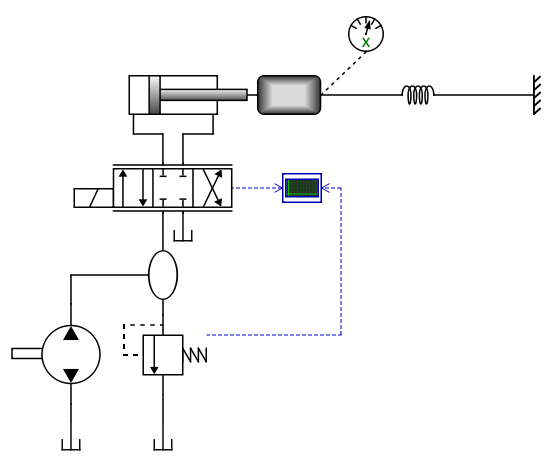
\includegraphics[height=7cm]{gfx/simulink/model2.png}

%Lägg till interfacekomponenter (och döp dem) (bild)

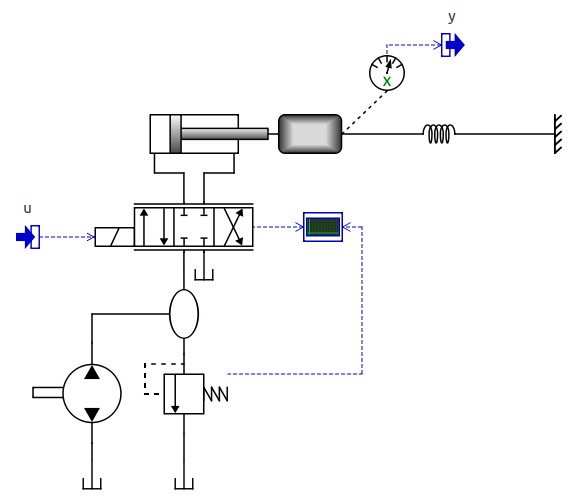
\includegraphics[height=7.593478263cm]{gfx/simulink/model3.png}

%Skapa en tom mapp

%Exportera till den tomma mappen

%Starta Matlab

%Gå till den tomma mappen

%Kör kompileringsskriptet

%Starta Simulink

%Lägg till ett S-functionblock

%Välj S-funktionen från Hopsan, nu ska det se ut så här (bild)

%Bygg en enkel P-regulator i Simulink

%Simulera

%Plotta

%Om du vill: jämför genom att göra samma sak i Hopsan



%\icon{0}{gfx/Hopsan-Simulate.png}{Simulate current project (Ctrl-Shift-S)}

\end{enumerate}

\end{document}